\section{Related Work}

\begin{frame}
	\frametitle{Related Work}
	
	\Large
	
	\vspace{0.6cm}
	
	Magnetic resonance imaging does have a good ability for differentiating between soft tissues like
	the brain.
	
	\vspace{0.2cm}
	
	Multiple approaches successfully used MRI brain scans for abnormality/normality Alzheimer
	assessment \cite{DeVos16,Devanand07,Wolz11}.
	
	\vspace{0.2cm}
	
	Many other imaging modalities exists in order to study Alzheimer and other brain diseases such as
	computed tomography (CT) and positron emission tomography (PET).
	
	\vspace{0.2cm}
	
	\tiny
	
	\cite{DeVos16} F. de Vos \emph{et al.}, ``Combining multiple anatomical MRI measures improves
	Alzheimer's disease classification'', Human Brain\\ \hspace{0.25cm} Mapping, 2016
	
	\cite{Devanand07} D. P. Devanand \emph{et al.}, ``Hippocampal and entorhinal atrophy in mild
	cognitive impairment prediction of Alzheimer disease'',\\ \hspace{0.25cm} Journal on Neurology,
	2007
	
	\cite{Wolz11} R. Wolz \emph{et al.}, ``Multi-method analysis of MRI images in early diagnostics of
	Alzheimer's disease'', PloS One, 2011
\end{frame}

\begin{frame}
	\frametitle{Related Work}
	
	\Large
	
	\vspace{1cm}
	
	We \emph{discuss} methods that are mostly related with MRI.
	
	\vspace{0.3cm}
	
	Anandh \emph{et al.} \cite{Anandh16} propose to \textbf{differentiate} Mild Cognitive Impairment
	(MCI), Condition Normal (CN) and AD subjects from MRI scans using an approach based on
	\textbf{Laplace-Beltrami eigenvalue} shape descriptors. Those descriptors are identified and their
	performance is \textbf{analysed} using linear Support Vector Machine (SVM) classifier.
	
	\vspace{0.72cm}
	
	\tiny
	
	\cite{Anandh16} K. R. Anandh \emph{et al.}, ``A method to differentiate mild cognitive impairment
	and Alzheimer in MR images using eigen value\\ \hspace{0.25cm} descriptors'', Journal on Medical
	Systems, 2016
\end{frame}

\begin{frame}
	\frametitle{Related Work}
	
	\Large
	
	\vspace{1cm}
	
	\begin{itemize}
		\item Beheshti \emph{et al.} \cite{Beheshti16} describe the use of \textbf{t-test} based
			  feature-ranking approach as part of their feature extraction procedure, where the number
			  of \textbf{top features} is determined using the Fisher criterion
		\vspace{0.2cm}
		\item Plocharski \emph{et al.} \cite{Plocharski16} design a technique to extract \textbf{sulcal
			  features} by means of computing a sulcal medial surface for AD/CN classification
	\end{itemize}
	
	\vspace{0.7cm}
	
	\tiny
	
	\cite{Beheshti16} I. Beheshti \emph{et al.}, ``Feature-ranking-based Alzheimer's disease
	classification from structural MRI'', Journal on Magnetic\\ \hspace{0.25cm} Resonance Imaging, 2016
	
	\cite{Plocharski16} M. Plocharski \emph{et al.}, ``Extraction of sulcal medial surface and
	classification of Alzheimer's disease using sulcal features'',\\ \hspace{0.25cm} Journal on
	Computer Methods and Programs in Biomedicine, 2016
\end{frame}

\begin{frame}
	\frametitle{Related Work}
	
	\Large
	
	\vspace{0.6cm}
	
	Daliri \cite{Daliri12} proposes an automated method for diagnosing Alzheimer's disease from brain
	MRI scans, where a \textbf{computer vision feature extractor} - called \emph{SIFT} \cite{Lowe04} -
	is used to extract features for tackling the classification task.
	
	\begin{center}
		\begin{tikzpicture}
			\node at (0,0) [draw=red,ultra thick,inner sep=0pt]
			{
				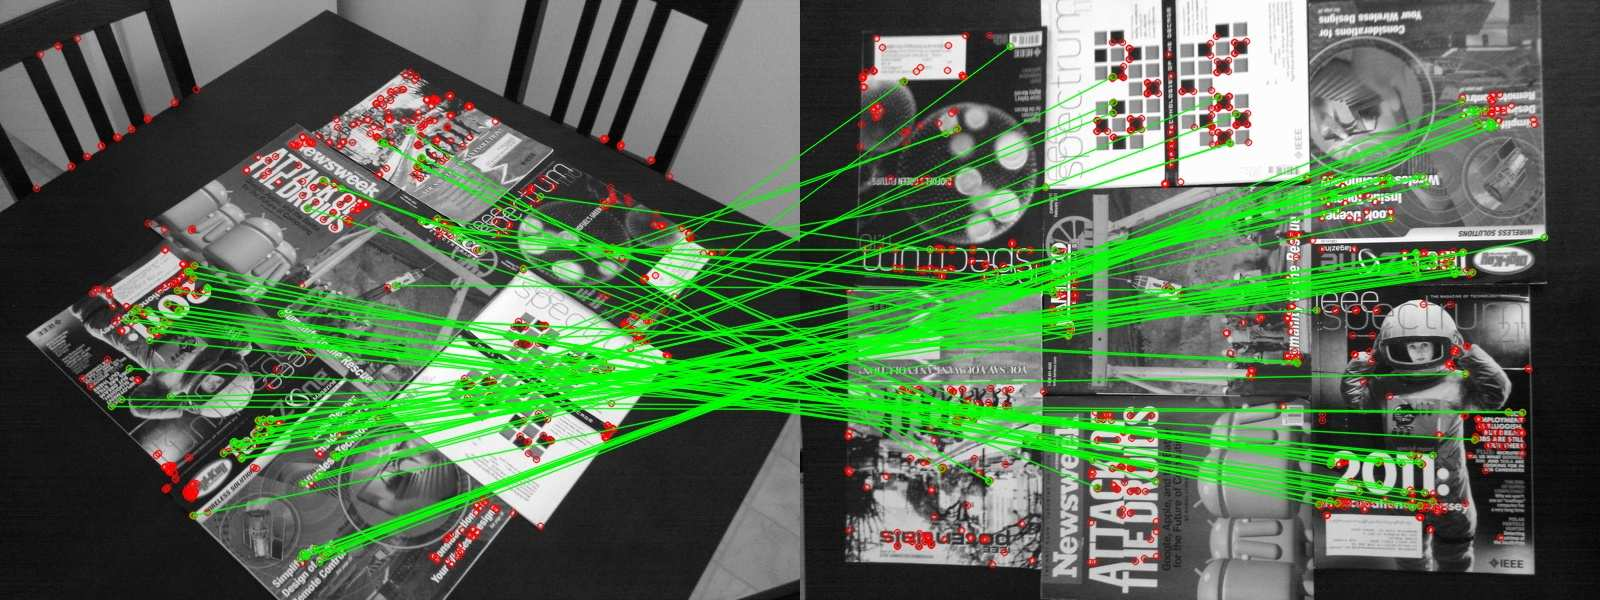
\includegraphics[scale=0.145]{Figures/SIFT}
			};
		\end{tikzpicture}
	\end{center}
	
	\vspace{0.02cm}
	
	\tiny
	
	\cite{Daliri12} M. R. Daliri, ``Automated diagnosis of Alzheimer disease using the scale-invariant
	feature transforms in magnetic resonance\\ \hspace{0.25cm} images'', Journal on Medical Systems,
	2012
	
	\cite{Lowe04} D. G. Lowe \emph{et al.}, ``Distinctive image features from scale-invariant
	keypoints'', Journal on Computer Vision, 2004
\end{frame}
